%-----------------------------------------------------------------------
% Beginning of chapter.tex
%-----------------------------------------------------------------------
%
%  This is a sample file for use with AMS-LaTeX.  It provides an example
%  of how to set up a file for a book to be typeset with AMS-LaTeX.
%
%  This is the driver file.  Separate chapters should be included at
%  the end of this file.
%
%  ***** DO NOT USE THIS FILE AS A STARTER FOR YOUR BOOK. *****
%  Follow the guidelines in the file chapter.template.
%
%%%%%%%%%%%%%%%%%%%%%%%%%%%%%%%%%%%%%%%%%%%%%%%%%%%%%%%%%%%%%%%%%%%%%%%%

\documentclass[11pt,a4paper]{memoir}
\chapterstyle{demo}
\epigraphfontsize{\small\itshape}
\setlength\epigraphwidth{8cm}
\setlength\epigraphrule{0pt}
\epigraphfontsize{\small\itshape}
%\includeonly{preface,chap1,biblio}

%\numberwithin{section}{chapter}
%\numberwithin{equation}{chapter}

% Include macros here
%=================================================
% Packages
%=================================================

%\usepackage{fixltx2e}
\usepackage[usenames,dvipsnames]{xcolor}
%\usepackage{fancyhdr}
\usepackage{amsmath,amsfonts,amsbsy,amsgen,amscd,mathrsfs,amssymb,amscd}
\usepackage{amsthm}
\usepackage{bm}
\usepackage{url}
\usepackage[UKenglish]{babel}
\usepackage{eurosym}
\usepackage{tikz}
\usepackage{caption}
\usetikzlibrary{matrix,arrows,shapes,calc,3d}
\usepackage{tikz-3dplot}
\tdplotsetmaincoords{60}{110}
\pgfmathsetmacro{\rvec}{.8}
\pgfmathsetmacro{\thetavec}{30}
\pgfmathsetmacro{\phivec}{60}

\tikzset{mynode/.style = {
    % The shape
    circle,
    % The size
    minimum size=2pt,
    % The color
    draw=black, fill=black}
}
\tikzset{vertex/.style={shape=circle, % style for a vertex
                        minimum size=3pt,
                        fill=gray,
                        inner sep = 0pt}}  

% \usepackage{3dplot}
% \tdplotsetmaincoords{60}{110}
%\usepackage{subfig}
\usepackage{microtype}
\usepackage{enumitem}
\usepackage{listings}
\definecolor{darkblue}{rgb}{0,0,.75}

\usepackage[many]{tcolorbox}
\tcbuselibrary{listings}

\definecolor{light-gray}{rgb}{0.96,0.96,0.96}
\definecolor{kwgreen}{rgb}{0,0.5,0}
\definecolor{cogreen}{rgb}{0.25,0.5,0.5}
\definecolor{mygreen}{rgb}{0,0.5,0.125}
\definecolor{equalsign}{rgb}{0.66,0.13,1}
\definecolor{darkred}{rgb}{0.75,0.16,0.37}

\lstloadlanguages{Python} %use listings with Python
%\lstset{literate={==}{{\color{equalsign}==}} {\*}{{\color{equalsign}\*}}}
%\lstnewenvironment{PseudoCode}[1][]
% the space reserved between for the ``In'' numbers and the code
\newlength\inwd
\setlength\inwd{1.7cm}

\newcounter{ipythcntr}

\newtcblisting{ipythonnb}[1][\theipythcntr]{
  enlarge left by=\inwd,
  width=\linewidth-\inwd,
  enhanced,
  boxrule=0.4pt,
  boxsep=0pt,
  left=2pt,
  top=0pt,
  colback=light-gray,
  listing only,
  top=0pt,
  bottom=0pt,
  arc=1pt,
  overlay={
    \node[
      anchor=north east,
      text width=\inwd,
      font=\footnotesize\ttfamily\color{blue!50!black},
      inner ysep=2.5mm,
      inner xsep=0pt,
      outer sep=0pt
      ] 
      at (frame.north west)
      {\stepcounter{ipythcntr}In [#1]:};
  }
  listing style=Python,
  listing options={
    basicstyle=\scriptsize\ttfamily\color{black},
    language=Python,
    escapechar=£,
    showstringspaces=false,
    commentstyle=\color{cogreen},
    keywordstyle=\bfseries\color{kwgreen},
    stringstyle=\color{darkred},
    numberstyle=\color{kwgreen},
    identifierstyle=\color{black},
    %emph={from,import,as},          % Custom highlighting
    otherkeywords={0,1,2,3,4,5,6,7,8,9,\*,==,<=,>=,+,-,\%},
    emph={*,==,<=,>=,+,-,\%},    
    emphstyle=\color{equalsign},
    extendedchars=true,
  },
}

\newtcblisting{ipythonnbout}[1][\theipythcntr]{
  enlarge left by=\inwd,
  width=\linewidth-\inwd,
  enhanced,
  boxrule=0pt,
  boxsep=0pt,
  left=2pt,
  top=0pt,
  colback=white,
  listing only,
  top=0pt,
  bottom=0pt,
  frame hidden,
  overlay={
    \node[
      anchor=north east,
      text width=\inwd,
      font=\footnotesize\ttfamily\color{red},
      inner ysep=2.5mm,
      inner xsep=0pt,
      outer sep=0pt
      ] 
      at (frame.north west)
      {\stepcounter{ipythcntr}Out [#1]:};
  }
  listing style=Python,
  listing options={
    basicstyle=\scriptsize\ttfamily\color{black},
    language=Python,
    escapechar=£,
    showstringspaces=false,
    commentstyle=\color{cogreen},
    keywordstyle=\bfseries\color{kwgreen},
    stringstyle=\color{darkred},
    numberstyle=\color{kwgreen},
    identifierstyle=\color{black},
    %emph={from,import,as},          % Custom highlighting
%    otherkeywords={as,0,1,2,3,4,5,6,7,8,9,\*,==,<=,>=,+,-},
%    emph={*,==,<=,>=,+,-},    
%    emphstyle=\color{equalsign},
    extendedchars=true,
    %literate={#}{{\#}},
  },
}

\newtcblisting{ipythonnboutno}{
  enlarge left by=\inwd,
  width=\linewidth-\inwd,
  enhanced,
  boxrule=0pt,
  boxsep=0pt,
  left=2pt,
  top=0pt,
  colback=white,
  listing only,
  top=0pt,
  bottom=0pt,
  frame hidden,
  overlay={
    \node[
      anchor=north east,
      text width=\inwd,
      font=\footnotesize\ttfamily\color{red},
      inner ysep=2.5mm,
      inner xsep=0pt,
      outer sep=0pt
      ] 
      at (frame.north west)
      {};
  }
  listing style=Python,
  listing options={
    basicstyle=\scriptsize\ttfamily\color{black},
    language=Python,
    escapechar=£,
    showstringspaces=false,
    commentstyle=\color{cogreen},
    %keywordstyle=\bfseries\color{kwgreen},
    stringstyle=\color{darkred},
    numberstyle=\color{kwgreen},
    identifierstyle=\color{black},
    %emph={from,import,as},          % Custom highlighting
    %otherkeywords={as,0,1,2,3,4,5,6,7,8,9,\[,\]},
    %emph={[,]},    
    %emphstyle=\color{black},
    extendedchars=true,
    %literate={#}{{\#}},
  },
}


%{\lstset{language=Matlab,basicstyle=\small, keywordstyle=\color{darkblue},numbers=none,xleftmargin=.04\textwidth,mathescape,frame=single,#1}}
%{}
%\usepackage[]{algorithm2e}
%\usepackage{mcode}
\usepackage{multicol}

%\usepackage[draft]{changes}
%\definechangesauthor[color=blue]{ml}
%\definechangesauthor[color=red]{da}
% \usepackage{trackchanges}
% \addeditor{ml}
% \addeditor{da}

\definecolor{dark-gray}{gray}{0.3}
\definecolor{dkgray}{rgb}{.4,.4,.4}
\definecolor{dkblue}{rgb}{0,0,.5}
\definecolor{medblue}{rgb}{0,0,.75}
\definecolor{rust}{rgb}{0.5,0.1,0.1}

\usepackage[colorlinks=true]{hyperref}
\hypersetup{urlcolor=Blue}
\hypersetup{citecolor=Black}
\hypersetup{linkcolor=dark-gray}

%\usepackage{setspace}
\usepackage{graphicx}
%\usepackage{multicol}
\usepackage{booktabs,longtable,tabu} % Nice tables
\setlength{\tabulinesep}{1pt}
\usepackage{multirow} % More control over tables
\usepackage{float}
\usepackage[T1]{fontenc}
%\usepackage{quotchap}

% Fonts
\usepackage{times}
%\usepackage{fourier}
%\usepackage[no-math]{fontspec}
%\setmainfont{optima}
%\usepackage{charter}
\usepackage{bm} % boldmath must be called after the package

%=================================================
% Paths
%=================================================

\graphicspath{{figures/}}

%=================================================
% Formatting
%=================================================

%\sloppy % Helps with margin justification

%%% Further font changes
\newcommand{\lang}{\textit}
\newcommand{\titl}{\textsl}
\newcommand{\term}{\emph}

%%% Equation numbering
\numberwithin{equation}{section} 

%%% Typesetting
\providecommand{\mathbold}[1]{\bm{#1}}  % Must be after 'fourier'
                                % package loads
%%% Annotations
\newcommand{\notate}[1]{\textcolor{red}{\textbf{[#1]}}}

%=================================================
% Theorem environment
%=================================================

\newtheorem{bigthm}{Theorem}
\renewcommand{\thebigthm}{\Roman{bigthm}}

\newtheorem{theorem}{Theorem}[section]
\newtheorem{lemma}[theorem]{Lemma}
\newtheorem{sublemma}[theorem]{Sublemma}
\newtheorem{proposition}[theorem]{Proposition}
\newtheorem{fact}[theorem]{Fact}
\newtheorem{result}[theorem]{Result}
\newtheorem{conjecture}[theorem]{Conjecture}
\newtheorem{corollary}[theorem]{Corollary}

\newtheorem{problem}[theorem]{Problem}
\newtheorem{solution}[theorem]{Solution}

\theoremstyle{definition}

\newtheorem{definition}[theorem]{Definition}
\newtheorem{example}[theorem]{Example}
\newtheorem{remark}[theorem]{Remark}

\newenvironment{mainthm}{\par\textsc{Main theorem.}\it}{\par}
\renewcommand{\thebigthm}{\Alph{bigthm}}

%=================================================
% Symbols
%=================================================

%%% Old symbols with new names
\newcommand{\oldphi}{\phi}
\renewcommand{\phi}{\varphi}

\newcommand{\eps}{\varepsilon}
\newcommand{\e}{\varepsilon}

%\newcommand{\oldmid}{\mid}
\renewcommand{\mid}{\mathrel{\mathop{:}}} 

%%% New symbols
\newcommand{\defby}{\overset{\mathrm{\scriptscriptstyle{def}}}{=}}
\newcommand{\half}{\tfrac{1}{2}}
\newcommand{\third}{\tfrac{1}{3}}

\newcommand{\sumnl}{\sum\nolimits}

\newcommand{\defeq}{\ensuremath{\mathrel{\mathop{:}}=}} % Definition-equals
\newcommand{\eqdef}{\ensuremath{=\mathrel{\mathop{:}}}} % Equals-definition

%%% Constants
\newcommand{\cnst}[1]{\mathrm{#1}} 
\newcommand{\econst}{\mathrm{e}}
\newcommand{\iunit}{\mathrm{i}}

\newcommand{\onevct}{\mathbf{e}} % All ones vector
\newcommand{\zerovct}{\vct{0}} % Zero vector

\newcommand{\Id}{\mathbf{I}}
\newcommand{\onemtx}{\bm{1}}
\newcommand{\zeromtx}{\bm{0}}

%%% Sets
\newcommand{\coll}[1]{\mathscr{#1}}
\newcommand{\sphere}[1]{S^{#1}}
\newcommand{\ball}[1]{B^{#1}}
\newcommand{\Grass}[2]{\mathbb{G}(#1,#2)}
\providecommand{\mathbbm}{\mathbb} % In case we don't load bbm
\newcommand{\Rplus}{\mathbbm{R}_{+}}
\newcommand{\R}{\mathbbm{R}}
\newcommand{\C}{\mathbbm{C}}
\newcommand{\N}{\mathbbm{N}}
\newcommand{\FF}{\mathbbm{F}}
\newcommand{\struct}{\mathcal{S}}

% Group theory
\newcommand{\stab}{\mathrm{stab}}

% Algebra
\newcommand{\End}{\mathrm{End}}
\newcommand{\Hom}{\mathrm{Hom}}
\newcommand{\Mult}{\mathrm{Mult}}

% Set operations
\newcommand{\polar}{\circ}
\newcommand{\closure}{\overline}
\newcommand{\prtensor}{\,\hat{\otimes}\,}

%%% Real and complex analysis
\newcommand{\abs}[1]{\left\vert {#1} \right\vert}
\newcommand{\abssq}[1]{{\abs{#1}}^2}

\newcommand{\sgn}[1]{\operatorname{sgn}{#1}}
\newcommand{\real}{\operatorname{Re}}
\newcommand{\imag}{\operatorname{Im}}
\newcommand{\pos}{\operatorname{Pos}}
\newcommand{\shrink}{\operatorname{Shrink}}

\newcommand{\diff}[1]{\mathrm{d}{#1}}
\newcommand{\idiff}[1]{\, \diff{#1}}

\newcommand{\gradd}{\mathrm{grad }} % Conflicts w/SIAM styles?
\newcommand{\divv}{\mathrm{div }}
\newcommand{\subdiff}{\partial}

%%% Optimization

\newcommand{\minimize}{\text{minimize}\quad}
\newcommand{\maximize}{\text{maximize}\quad}
\newcommand{\subjto}{\quad\text{subject to}\quad}
\newcommand{\find}{\text{find}\quad}
\newcommand{\suchthat}{\quad\text{such that}\quad}

\newcommand{\argmin}{\operatorname*{arg\; min}}
\newcommand{\argmax}{\operatorname*{arg\; max}}
\newcommand{\dom}{\mathrm{dom} }

%%% Probability & measure

\newcommand{\Prob}{\mathbbm{P}}
\newcommand{\Probe}[1]{\Prob\left({#1}\right)}
\newcommand{\Expect}{\operatorname{\mathbb{E}}}

\newcommand{\St}{\operatorname{St}}

%\newcommand{\normal}{\textsc{Normal}}
\newcommand{\normal}{N}
\newcommand{\uniform}{\textsc{Uniform}}
\newcommand{\erf}{\operatorname{erf}}

\DeclareMathOperator{\rvol}{rvol}
\DeclareMathOperator{\Var}{Var}
\DeclareMathOperator{\Gl}{Gl}
\newcommand{\diag}{\operatorname{diag}}

%%% Vector and matrix operators
\newcommand{\vct}[1]{\mathbold{#1}}
\newcommand{\mtx}[1]{\mathbold{#1}}
\newcommand{\Eye}{\mathbf{I}}

\newcommand{\transp}[1]{#1^{T}}
\newcommand{\trans}{\top}
\newcommand{\adj}{*}
\newcommand{\psinv}{\dagger}

\newcommand{\lspan}[1]{\operatorname{span}{#1}}

\newcommand{\range}{\operatorname{range}}
\newcommand{\colspan}{\operatorname{colspan}}

%\newcommand{\rank}{\operatorname{rank}}
\newcommand{\nullity}{\operatorname{null}}
%\newcommand{\ker}{\operatorname{ker}}
\newcommand{\im}{\operatorname{im}}
%\newcommand{\span}{\operatorname{span}}

%\newcommand{\diag}{\operatorname{diag}}
\newcommand{\trace}{\operatorname{tr}}

\newcommand{\supp}[1]{\operatorname{supp}(#1)}
\newcommand{\sign}[1]{\operatorname{sign}(#1)}

\newcommand{\smax}{\sigma_{\max}}
\newcommand{\smin}{\sigma_{\min}}

\newcommand{\nnz}{\operatorname{nnz}}
\renewcommand{\vec}{\operatorname{vec}}

\newcommand{\Proj}{\ensuremath{\mtx{\Pi}}} % Projection operator

%%% Semidefinite orders
\newcommand{\psdle}{\preccurlyeq}
\newcommand{\psdge}{\succcurlyeq}

\newcommand{\psdlt}{\prec}
\newcommand{\psdgt}{\succ}

%%% Mensuration: inner products and norms

% TeX does not like either \newcommand or \renewcommand for these
% two macros.  There is probably a good reason not to use them via
% \def, but I don't know it.  
%\newcommand{\<}{\langle} 
%\newcommand{\>}{\rangle}
\newcommand{\ip}[2]{\langle {#1}, {#2} \rangle}
% --deleted the \left and \right-- Dennis
% \newcommand{\ip}[2]{\left\langle {#1},\ {#2} \right\rangle}
\newcommand{\absip}[2]{\abs{\ip{#1}{#2}}}
\newcommand{\abssqip}[2]{\abssq{\ip{#1}{#2}}}
\newcommand{\tworealip}[2]{2 \, \real{\ip{#1}{#2}}}

%\newcommand{\norm}[1]{\left\Vert {#1} \right\Vert}
\newcommand{\norm}[1]{\Vert {#1}\Vert}
\newcommand{\normsq}[1]{\norm{#1}^2}

\newcommand{\lone}[1]{\norm{#1}_{\ell_1}}
\newcommand{\smlone}[1]{\|#1\|_{\ell_1}}
\newcommand{\linf}[1]{\norm{#1}_{\ell_\infty}}
\newcommand{\sone}[1]{\norm{#1}_{S_1}}
\newcommand{\snorm}[1]{\sone{#1}}
\newcommand{\wnnorm}[1]{\norm{#1}_{*,\vct{w}}}
\newcommand{\wnnormd}[1]{\norm{#1}^*_{\vct{w}}}
\DeclareMathOperator{\dist}{dist}

% Fixed-size inner products and norms are useful sometimes
\newcommand{\smip}[2]{\bigl\langle {#1}, \ {#2} \bigr\rangle}
\newcommand{\smabsip}[2]{\bigl\vert \smip{#1}{#2} \bigr\vert}
\newcommand{\smnorm}[2]{{\bigl\Vert {#2} \bigr\Vert}_{#1}}

% Specific norms that are used frequently
\newcommand{\enormdangle}{{\ell_2}}
\newcommand{\enorm}[1]{\norm{#1}}
\newcommand{\enormsm}[1]{\enorm{\smash{#1}}}

\newcommand{\enormsq}[1]{\enorm{#1}^2}

\newcommand{\fnorm}[1]{\norm{#1}_{\mathrm{F}}}
\newcommand{\fnormsq}[1]{\fnorm{#1}^2}

\newcommand{\pnorm}[2]{\norm{#2}_{#1}}
%\newcommand{\snorm}[1]{\norm{#1}_*}

\newcommand{\triplenorm}[1]{\left\vert\!\left\vert\!\left\vert {#1} \right\vert\!\right\vert\!\right\vert} 

\newcommand{\flag}[2]{{#1 \brack #2}}

% Special cones
\newcommand{\Feas}{\mathcal{F}}
\newcommand{\Desc}{\mathcal{D}}

\newcommand{\sdim}{\delta}
\newcommand{\sdimw}{\delta^*}
% \newcommand{\sdimw}{\tilde{\delta}}
\newcommand{\ddt}[1]{\dot{#1}}
\DeclareMathOperator{\Circ}{Circ}

%%% Differential geometry
\newcommand{\Cinf}{C^{\infty}}
\newcommand{\Tensf}{\mathcal{T}}
\newcommand{\Vbundle}{\mathcal{X}}
\newcommand{\Christ}[3]{\Gamma_{{#1}{#2}}^{#3}}

% Stuff to be sorted in somewhere
\DeclareMathOperator{\Lip}{Lip}

\newcommand{\IR}{\mathbbm{R}}
\newcommand{\veps}{\varepsilon}
\newcommand{\mA}{\mathcal{A}}
\newcommand{\mB}{\mathcal{B}}
\newcommand{\mC}{\mathcal{C}}
\newcommand{\mD}{\mathcal{D}}
\newcommand{\mE}{\mathcal{E}}
\newcommand{\mI}{\mathcal{I}}
\newcommand{\mM}{\mathcal{M}}
\newcommand{\mN}{\mathcal{N}}
\newcommand{\mL}{\mathcal{L}}
\newcommand{\mV}{\mathcal{V}}
\newcommand{\bface}{\overline{\mathcal{F}}}
\newcommand{\face}{\mathcal{F}}
\newcommand{\relint}{\operatorname{relint}}
\newcommand{\relcl}{\operatorname{relcl}}
\newcommand{\cone}{\operatorname{cone}}
\newcommand{\lin}{\operatorname{lin}}
\newcommand{\Gr}{\operatorname{Gr}}
\newcommand{\powerset}{\mathscr{P}}
\newcommand{\hd}{{\operatorname{hd}}}
\newcommand{\inter}{{\operatorname{int}}}
\newcommand{\conv}{\operatorname{conv}}
\newcommand{\clconv}{\overline{\conv}}
\newcommand{\cl}{\operatorname{cl}}
\newcommand{\bd}{\operatorname{bd}}

\newcommand{\GL}{\operatorname{GL}}

% \newcommand{\tb}{\stackrel{0}{\to}}
\newcommand{\tb}{\,\,\mathring{\to}\,\,}
% \newcommand{\tdash}{\,\,\overset{e}{\to}\,\,}
% \newcommand{\tdash}{\,\,\overset{a}{\to}\,\,}
\newcommand{\tdash}{\overset{a}{\to}}

\newcommand{\K}{\mathcal{K}}
\newcommand{\B}{\mathcal{B}}
\newcommand{\F}{\mathcal{F}}
\newcommand{\D}{\mathcal{D}}
\renewcommand{\P}{\mathcal{P}}
\DeclareMathOperator{\id}{id}
\DeclareMathOperator{\gr}{gr}
\newcommand{\vp}{\varphi}
\newcommand{\maxp}{{\max}_p}
\DeclareMathOperator{\spa}{span}
\DeclareMathOperator{\vol}{vol}
\DeclareMathOperator{\ima}{im}
\DeclareMathOperator{\rk}{rk}

\newcommand{\Ren}{\mathcal{R}}
\newcommand{\T}{\mathcal{T}}
% ADJUST THE FOLLOWING
% \newcommand{\resTMP}[2]{#1,#2}
\newcommand{\resTMP}[2]{#1\to#2}
% 
\newcommand{\res}[3]{\vct{#1}_{\resTMP{#2}{#3}}}
\newcommand{\nres}[3]{\|\vct{#1}\|_{\resTMP{#2}{#3}}}
\newcommand{\sres}[3]{\sigma_{\resTMP{#2}{#3}}(\vct{#1})}
\newcommand{\csres}[3]{\overline{\sigma}_{\resTMP{#2}{#3}}(\vct{#1})}
\newcommand{\kres}[3]{\kappa_{\resTMP{#2}{#3}}(\vct{#1})}
% transpose
\newcommand{\rest}[3]{\vct{#1}^T_{\resTMP{#2}{#3}}}
\newcommand{\nrest}[3]{\|\vct{#1}^T\|_{\resTMP{#2}{#3}}}
\newcommand{\srest}[3]{\sigma_{\resTMP{#2}{#3}}(\vct{#1}^T)}
\newcommand{\csrest}[3]{\overline{\sigma}_{\resTMP{#2}{#3}}(\vct{#1}^T)}
\newcommand{\srestm}[3]{\sigma_{\resTMP{#2}{#3}}(-\vct{#1}^T)}
\newcommand{\krest}[3]{\kappa_{\resTMP{#2}{#3}}(\vct{#1}^T)}
\newcommand{\nresdag}[3]{\|\vct{#1}^\dagger\|_{\resTMP{#2}{#3}}}

\newcommand{\RCD}[3]{\Ren_{#2,#3}(\vct{#1})}
% \newcommand{\RCD}[3]{\Ren_{\resTMP{#2}{#3}}(\vct{#1})}

\newcommand{\DA}{\vct{\Delta A}}

%
\newcommand{\Rmm}{R_{\mathrm{mm}}}

\newcommand{\rbinom}[2]{\genfrac{[}{]}{0pt}{}{#1}{#2}}
\newcommand{\trbinom}[2]{{\textstyle\genfrac{[}{]}{0pt}{}{#1}{#2}}}

\newcommand{\comm}[1]{\textcolor{red}{\textbf{[#1]}}}
\newcommand{\rant}[1]{\textcolor{blue}{\textbf{[#1]}}}
%

\newcommand{\llangle}{\langle\hspace{-1.5pt}\langle}  % this is actually contained in mnsymbol, but loading this package causes trouble...
\newcommand{\rrangle}{\rangle\hspace{-1.5pt}\rangle}  % this is actually contained in mnsymbol, but loading this package causes trouble...

\newcommand{\Res}{\mathrm{Res}}
\newcommand{\Oh}{\mathcal{O}}
\newcommand{\Mbar}{\overline{M}}
\newcommand{\second}{\mathrm{II}}
\newcommand{\nablabar}{\overline{\nabla}}
\newcommand{\expm}{\mathrm{exp}}
\newcommand{\Rc}{\mathrm{Rc}}
\newcommand{\NJ}{\mathrm{NJ}}
% %\newcommand{\GL}[1]{\mathrm{GL}(#1)}

\newcommand{\cover}{\lessdot}

% Semidefinite programming
\newcommand{\Sym}{\mathcal{S}}
\newcommand{\SDP}{\mathcal{S}_+}
\newcommand{\psd}{\succeq}
\newcommand{\bdot}{\bullet}

%\renewcommand{\chaptername}{}
%\renewcommand{\thechapter}{}

\begin{document}
%\numberwithin{section}{chapter}
\numberwithin{equation}{chapter}
\numberwithin{theorem}{chapter}

\lstset{language=Matlab}

%\frontmatter
%\title{Convex Optimization}

%    Information for first author
%\author{Martin Lotz}
%    Address of record for the research reported here

%\address{School of Mathematics\\ The University of Manchester\\ Alan Turing Building, Oxford Road\\ Manchester M139PL}

%\email{martin.lotz@manchester.ed.uk}
%\urladdr{http://www.maths.manchester.ac.uk/\textasciitilde mlotz}

%\date{\today}

%\maketitle

%\newpage 

%\tableofcontents

%\include{preface}

\mainmatter

%\include{notation}
%-----------------------------------------------------------------------
% Beginning of chap2.tex
%-----------------------------------------------------------------------
%
%  AMS-LaTeX sample file for a chapter of a monograph, to be used with
%  an AMS monograph document class.  This is a data file input by
%  chapter.tex.
%
%  Use this file as a model for a chapter; DO NOT START BY removing its
%  contents and filling in your own text.
% 
%%%%%%%%%%%%%%%%%%%%%%%%%%%%%%%%%%%%%%%%%%%%%%%%%%%%%%%%%%%%%%%%%%%%%%%%


\chapter*{Lecture 13}
\addcontentsline{toc}{chapter}{Lecture 12}
\addtocounter{chapter}{3}
\addtocounter{section}{0}
%\numberwithin{section}{chapter}
\numberwithin{equation}{chapter}
\numberwithin{theorem}{chapter}

%\epigraph{}{--- \textup{}}

Primal-dual interior point methods aim to solve the problem
\begin{equation}\label{eq:standard}\tag{P}
 \minimize \ip{\vct{c}}{\vct{x}} \quad \subjto \mtx{A}\vct{x}=\vct{b}, \ \vct{x}\geq \zerovct
\end{equation}
for a matrix $\mtx{A}\in \R^{m\times n}, \vct{b}\in \R^m$ and $\vct{c}\in \R^n$, by applying Newton-type iterations to the optimality conditions of linear programming. More precisely, we have seen the following algorithm. Recall the feasible sets
\begin{align*}
 \mathcal{F} &= \{(\vct{x},\vct{y},\vct{s}) \mid \mtx{A}^{\trans}\vct{y}+\vct{s}=\vct{c}, \ \mtx{A}\vct{x}=\vct{b}, \ \vct{x}\geq \zerovct, \ \vct{s}\geq \zerovct\}\\
 \mathcal{F}^{\circ} &= \{(\vct{x},\vct{y},\vct{s}) \mid \mtx{A}^{\trans}\vct{y}+\vct{s}=\vct{c}, \ \mtx{A}\vct{x}=\vct{b}, \ \vct{x}> \zerovct, \ \vct{s}> \zerovct\}\\
\end{align*}
The a simple primal-dual interior point method can be described as follows.
\begin{itemize}
 \item Start with $(\vct{x}^{(0)},\vct{y}^{(0)},\vct{s}^{(0)})\in \mathcal{F}^{\circ}$;
 \item For each $k\geq 0$, compute the duality parameter
 \begin{equation*}
  \mu^{(k)} = \frac{1}{n} \sum_{i=1}^n x_is_i
 \end{equation*}
and choose $\sigma_k\in [\sigma_{\mathrm{min}},\sigma_{\mathrm{max}}]$. Solve
\begin{equation*}
 \begin{pmatrix}
  \zerovct & \mtx{A}^{\trans} & \mtx{I} \\
  \mtx{A} & \zerovct & \zerovct \\
  \mtx{S}^{(k)} & \zerovct & \mtx{X}^{(k)}
 \end{pmatrix}
\begin{pmatrix} \Delta\vct{x}\\ \Delta \vct{y}\\ \Delta\vct{s} \end{pmatrix} = \begin{pmatrix} \zerovct \\ \zerovct \\ -\vct{X}^{(k)}\mtx{S}^{(k)}\vct{e}+\sigma \mu^{(k)}\vct{e}\end{pmatrix}
\end{equation*}
and compute
\begin{equation*}
\begin{pmatrix} \vct{x}^{k+1}\\ \vct{y}^{k+1}\\ \vct{s}^{k+1}\end{pmatrix}= \begin{pmatrix} \vct{x}^{k}\\ \vct{y}^{k}\\ \vct{s}^{k}\end{pmatrix} +\alpha_k \begin{pmatrix} \Delta\vct{x}\\ \Delta \vct{y}\\ \Delta\vct{s} \end{pmatrix},
 \end{equation*}
for a small enough $\alpha_k>0$ to ensure non-negativity.
\end{itemize}

In each iteration, a Newton step is taken in the direction of the \textbf{path}. This is a curve in $\mathcal{F}^{\circ}$ defined as the set of solutions of
\begin{align}\label{eq:cpopt}
 \begin{split}
  \mtx{A}^{\trans}\vct{y}+\vct{s}-\vct{c} &= \zerovct\\
  \mtx{A}\vct{x}-\vct{b} & = \zerovct\\
  \mtx{X}\mtx{S}\vct{e} &= \tau \vct{e}\\
  \vct{x}&> \zerovct\\
  \vct{s}&> \zerovct,
 \end{split}
\end{align}
where $\tau>0$. 

\section{Path-following methods}
A path-following method tries to ensure that each iterate is {\em close} to the central path. What it means to be close to the central path depends on the neighbourhood we choose. Here, we will look at the (one-sided) $\infty$-norm neighbourhood
\begin{equation*}
\mathcal{N}_{-\infty}(\gamma) = \{(\vct{x},\vct{y},\vct{s})\in \mathcal{F}^{\circ} \mid x_is_i\geq \gamma \mu, \ 1\leq i\leq n\}
\end{equation*}
for some $\gamma\in (0,1]$ (say, $\gamma=10^{-3}$). In words, each $x_is_i$ has to be at least some small multiple of their average value. To see what this has to do with the $\infty$-norm neighbourhood, consider the set of $\vct{x}$ such that
\begin{equation*}
 \norm{\mtx{X}\mtx{S}\vct{e}-\mu \vct{e}}_\infty \leq (1-\gamma) \mu \ \Longleftrightarrow \ \forall 1\leq i\leq n, \ \gamma \mu \leq x_is_i \leq 2-\gamma,
\end{equation*}
and we are only interested in the lower inequality.

The so-called {\em long-step path-following} interior point method can then be described as follows.
\begin{itemize}
 \item Start with $(\vct{x}^{(0)},\vct{y}^{(0)},\vct{s}^{(0)})\in \mathcal{N}_{-\infty}(\gamma)$;
 \item For each $k\geq 0$, compute the duality parameter
 \begin{equation*}
  \mu^{(k)} = \frac{1}{n} \sum_{i=1}^n x_is_i
 \end{equation*}
and choose $\sigma_k\in [\sigma_{\mathrm{min}},\sigma_{\mathrm{max}}]$. Solve
\begin{equation*}
 \begin{pmatrix}
  \zerovct & \mtx{A}^{\trans} & \mtx{I} \\
  \mtx{A} & \zerovct & \zerovct \\
  \mtx{S}^{(k)} & \zerovct & \mtx{X}^{(k)}
 \end{pmatrix}
\begin{pmatrix} \Delta\vct{x}\\ \Delta \vct{y}\\ \Delta\vct{s} \end{pmatrix} = \begin{pmatrix} \zerovct \\ \zerovct \\ -\vct{X}^{(k)}\mtx{S}^{(k)}\vct{e}+\sigma \mu^{(k)}\vct{e}\end{pmatrix}
\end{equation*}
and compute
\begin{equation*}
\begin{pmatrix} \vct{x}^{k+1}\\ \vct{y}^{k+1}\\ \vct{s}^{k+1}\end{pmatrix}= \begin{pmatrix} \vct{x}^{k}\\ \vct{y}^{k}\\ \vct{s}^{k}\end{pmatrix} +\alpha_k \begin{pmatrix} \Delta\vct{x}\\ \Delta \vct{y}\\ \Delta\vct{s} \end{pmatrix},
 \end{equation*}
for a small enough $\alpha_k\in [0,1]$ is the largest value such that $(\vct{x}^{(k+1)},\vct{y}^{(k+1)},\vct{s}^{(k+1)})\in \mathcal{N}_{-\infty}(\gamma)$.
\end{itemize}

\begin{remark}
 As noted at the end of Lecture 12, to find an initial point in $\mathcal{F}^{\circ}$ might not be trivial. In practice one can therefore also use the algorithm described above using {\em infeasible} points, though in this case we have to make sure that the residual norms $\norm{\vct{b}-\mtx{A}\vct{x}}$ and $\norm{\vct{c}-\vct{s}-\mtx{A}^{\trans}\vct{y}}$ remain bounded.
\end{remark}

\subsection{Visualising the algorithm}
The feasible set $\mathcal{F}^{\circ}$ usually lives in a space that can't be easily visualised, but if the dual version is two-dimensional,
\begin{equation*}
 \{\vct{y}\in \R^2 \mid \mtx{A}^{\trans}\vct{y}+\vct{s}=\vct{c}, \ \vct{s}\geq \zerovct\},
\end{equation*}
then we have a chance to see how the trajectories of the iterates in $\vct{y}$ look like.
Consider, for example, the linear programming problem whose dual is given by
\begin{align*}
\maximize & y_1+y_2\\
\subjto & 0.2py_1+y_2+s_p = 1+0.01p^2, \ 0\leq p\leq 10.
\end{align*}
The points $\vct{y}=(0,0)^{\trans}$, $\vct{x}=(1,\dots,1)^{\trans}/11$ and $\vct{s}=\vct{c}-\mtx{A}^{\trans}\vct{y}$ are strictly feasible starting points. The trajectory in the $\vct{y}$-plane of the algorithm (red path) and the constraint equations (blue lines) are given in the following diagram, where the parameter $\sigma=0.5$ was used.
\begin{figure}[h!]
\centering
 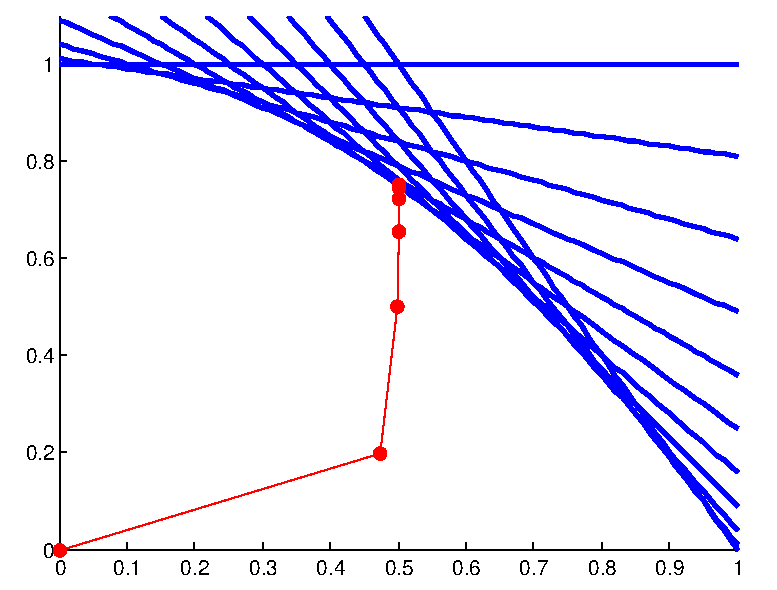
\includegraphics[width=0.7\textwidth]{images/lect12_cropped.pdf}
 \caption{Trajectory of long-step path-following in the $y_1-y_2$ plane.}\label{fig:fig1}
\end{figure}
It is instructive to play around with the parameter $\sigma$ and to try to determine the form of the central path in this example.

Another way to visualise the trajectory is to plot the pairs $x_is_i$ and $x_jy_j$ against each other.
Figure~\ref{fig:fig2} shows the trajectory of the above example in the $x_2s_2-x_5s_5$ plane. Note that the  central path, plotted in blue, is trivial in these coordinates, as it is defined by the property of the $x_is_i=\tau$ being equal.
\begin{figure}[h!]
\centering
 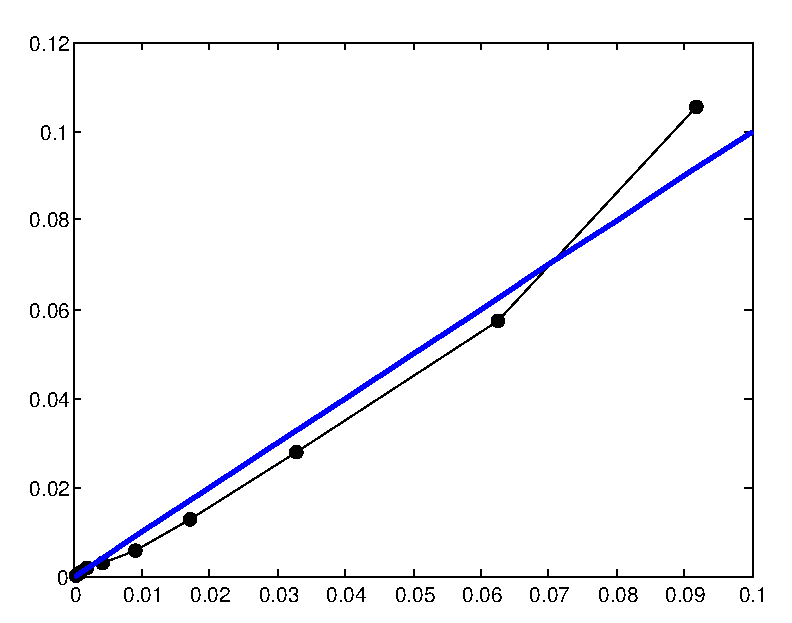
\includegraphics[width=0.7\textwidth]{images/lect12b_cropped.pdf}
 \caption{Trajectory and central path in $x_2s_2-x_5s_5$ coordinates.}\label{fig:fig2}
\end{figure}

\section{Analysis of Path-following}
In the analysis of the long-step path-following algorithm, it is enough to establish that the duality measure $\mu^{(k)}$ converges to $0$ as $k\to \infty$. The reason is that $\mu=0$ forces all the products $x_is_i=0$, and since by design the other constraints are satisfied, this means that the sequence of points converges to a solution. The first theorem tells us that the $\mu_k$ decrease as $k$ increases. An elementary proof is given in Theorem 14.3 in Nocedal and Wright. It depends crucially on the assumption that the iterates remain inside the neighbourhood $\mathcal{N}_{-\infty}(\gamma)$ of the central path.

\begin{theorem}
 Given parameters $\gamma$, $\sigma_{\mathrm{min}}$ and $\sigma_{\mathrm{max}}$, there is a constant $\delta>0$, independent of $n$, such that
 \begin{equation}\label{thm:1}
  \mu_{k+1}\leq \left(1-\frac{\delta}{n}\right) \mu_k.
 \end{equation}
\end{theorem}

The next theorem gives a bound on the number of iterations needed to reduce the duality measure beyond any given $\e$.

\begin{theorem}
 Let $\e>0$ and $\gamma\in (0,1)$. Let $(\vct{x}^{(0)},\vct{y}^{(0)},\vct{s}^{(0)})\in \mathcal{N}_{-\infty}(\gamma)$ be a starting point such that the duality measure satisfies $\mu^{(0)}\leq \e^{-\kappa}$ for some constant $\kappa$. Then there is an index $K=O(n\log (1/\e))$ such that for all $k>K$,
 \begin{equation*}
  \mu_k \leq \e.
 \end{equation*}
In particular, the long-step path-following algorithm converges.
\end{theorem}

\begin{proof}
Repeatedly applying~\eqref{thm:1}, we get
\begin{equation*}
 \mu_{k} \leq \left(1-\frac{\delta}{n}\right)^k \mu_0.
\end{equation*}
Taking logarithms on both sides,
 \begin{align*}
  \log \mu_{k}\leq k \log\left(1-\frac{\delta}{n}\right)+\log \mu_0 
  &\leq k \log\left(1-\frac{\delta}{n}\right)+\kappa \log\left(\frac{1}{\e}\right)\\
  &\leq k\frac{-\delta}{n}+\kappa\log\left(\frac{1}{\e}\right).
 \end{align*}
We have $\mu_k<\e$ if 
\begin{equation*}
 -k\frac{\delta}{n}+\kappa \left(\frac{1}{\e}\right) \leq \log \e,
\end{equation*}
of equivalently, if 
\begin{equation*}
 k\geq (1+\kappa)\frac{n}{\delta}\log\left(\frac{1}{\e}\right)=K.
\end{equation*}
This was to be shown.

\end{proof}



% %-----------------------------------------------------------------------
% % End of chap1.tex
% %-----------------------------------------------------------------------


%\appendix
%\include{appendix1}

%\backmatter
%\include{biblio}
%\include{index}
\end{document}

%-----------------------------------------------------------------------
% End of chapter.tex
%-----------------------------------------------------------------------
